%!TEX root = ../../main.tex

\chapter{Fazit und Ausblick}
Aufgrund der technischen Mängel und Probleme der Sensoren, welche in dieser Studienarbeit verwendet wurden, war es nicht möglich, das erhoffte Ergebnis der Arbeit zu erzielen.
Im Folgenden werden deshalb Möglichkeiten und Empfehlungen aufgezeigt, die unterstützend für ein mögliches, weiterführendes Projekt sein sollen.

Eine deutliche Empfehlung ist der Wechsel des, in dieser Studienarbeit eingesetzten, \ac{9-DOF} Sensors.
Für dieses Experiment ist ein Beschleunigsungssensor notwendig, welcher mit einer höheren Taktrate arbeiten kann.
Beispielsweise wird hierfür der Bosch BMA180, der unter anderem Anwendung in Drohnen findet, näher untersucht.
Dies ist ein dreiachsiger Beschleunigungssensor, welcher intern mit einer maximalen Messgeschwindigkeit von 1200 \ac{Hz} arbeiten kann.
Der Sensor ist somit in der Lage, alle 417$\mu$s eine neue Messreihe zu liefern.
Hiermit sind bei einer Umdrehungszeit von circa 24ms bis zu 48 Messergebnisse möglich, welche wahrscheinlich ausreichend sind für eine Aussage über die Unwuchtdetektion und -lokalisierung \cite{bosch_bma180}. \\
Eine weitere Möglichkeit den Beschleunigungssensor zu ersetzen, ist eventuell der Einsatz einer inertialen Messeinheit (englisch \textit{inertial measurement unit}, IMU).
Dies ist meist eine räumliche Kombination von mehreren Sensoren, welche auch Einsatz in heutigen Drohnen finden.
Ob diese den, für die Studienarbeit benötigten, Verwendungszweck erfüllen ist nicht bekannt und müsste für ein weiterführendes Projekt erst genauer recherchiert werden.

Des Weiteren sollte eine Lösung gefunden werden, die es erlaubt, beide Propellerblätter des Rotors unabhängig voneinander identifizieren zu können.
Zudem muss diese weiterhin in der Lage sein, dem \emph{Arduino} zuverlässige Interrupts nach dem Stand-Alone-Prinzip senden zu können.
Dadurch wird eine deutliche Erhöhung der Genauigkeit im Bereich der Unwuchtlokalisierung erwartet.

Wie anfangs erwähnt, sollte die Ausgabe der Unwuchtanalyse auf einem \ac{TFT-Display} stattfinden.
Da es jedoch nicht möglich war, die Unwucht zu detektieren und zu lokalisieren, wurde die Verwendung des \ac{TFT-Display}s in dieser Arbeit nicht behandelt.
Die Ansteuerung des Displays hingegen wurde exemplarisch durchgeführt.
Eine schematische Darstellung, wie der komplette Aufbau der Hardware aussehen könnte, ist in Abbildung \ref{fig:schema_hardware_future} dargestellt.

\begin{figure}[H]
	\centering
	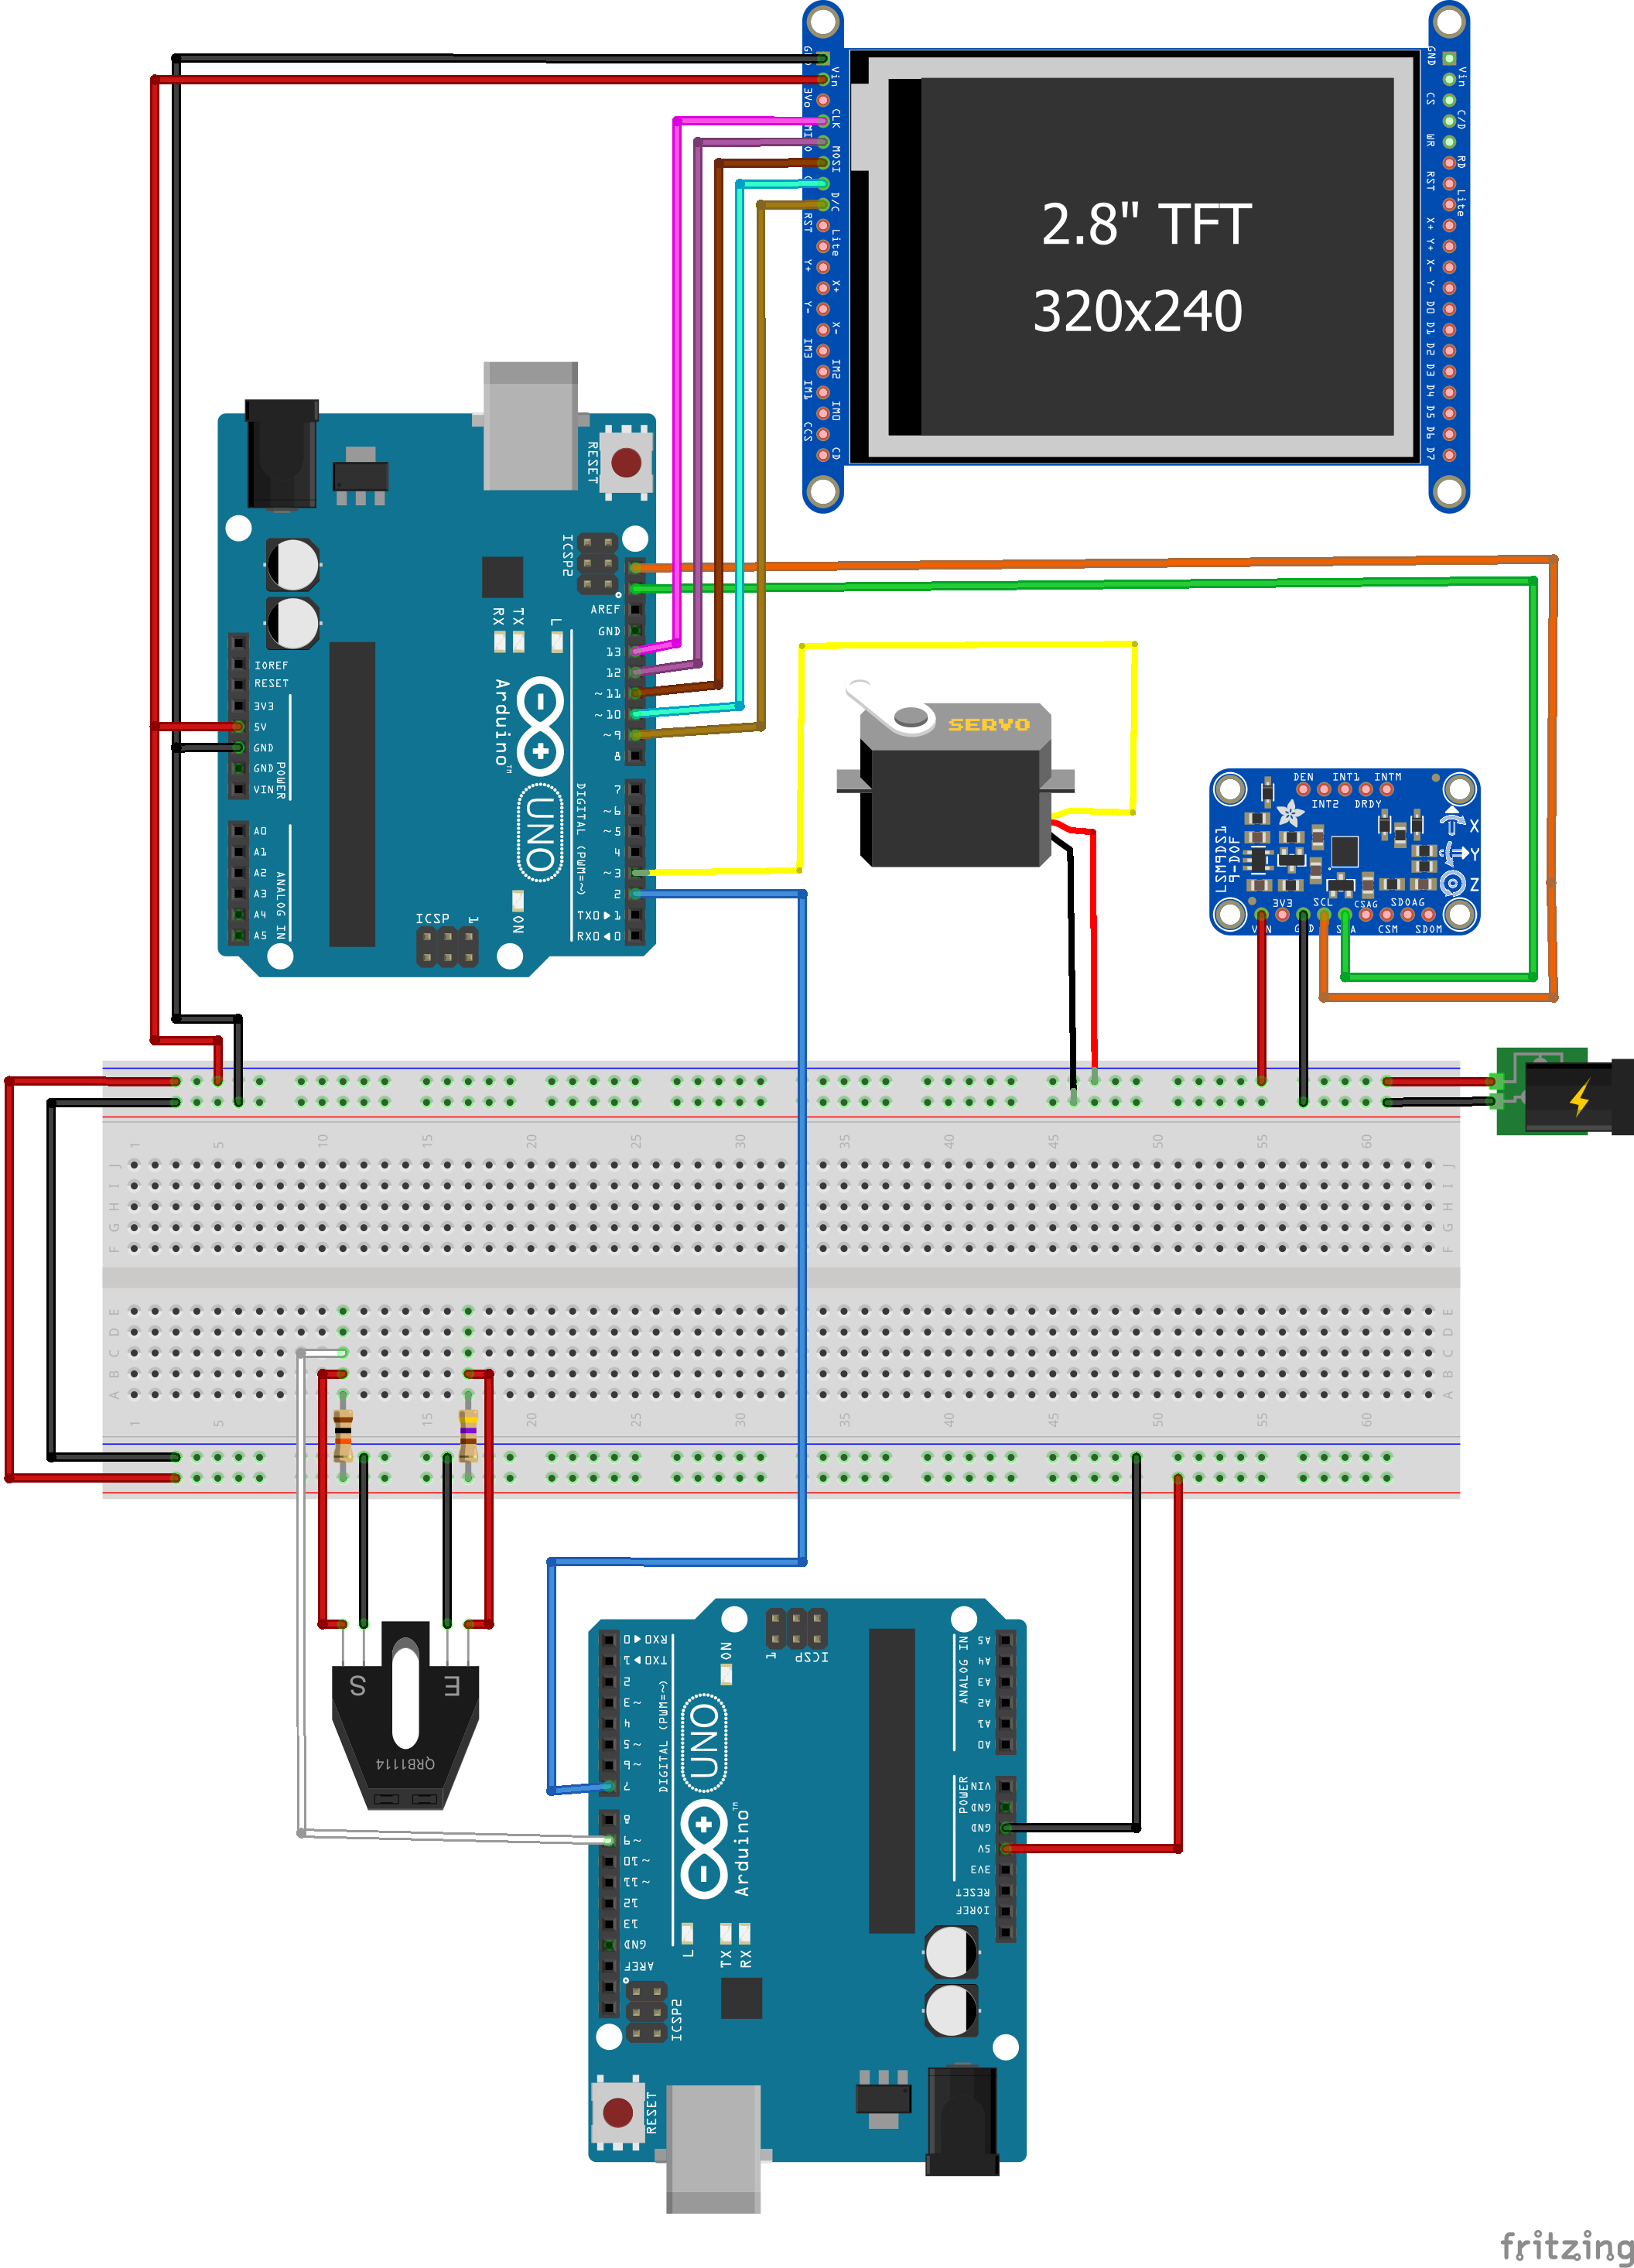
\includegraphics[width=10cm]{images/chapter/05/hardware-layout_future.png}
	\caption{Schematische Darstellung des Hardwaremodells mit TFT-Display}
	\label{fig:schema_hardware_future}
\end{figure}
